
\begin{figure*}[t]
  \centering
  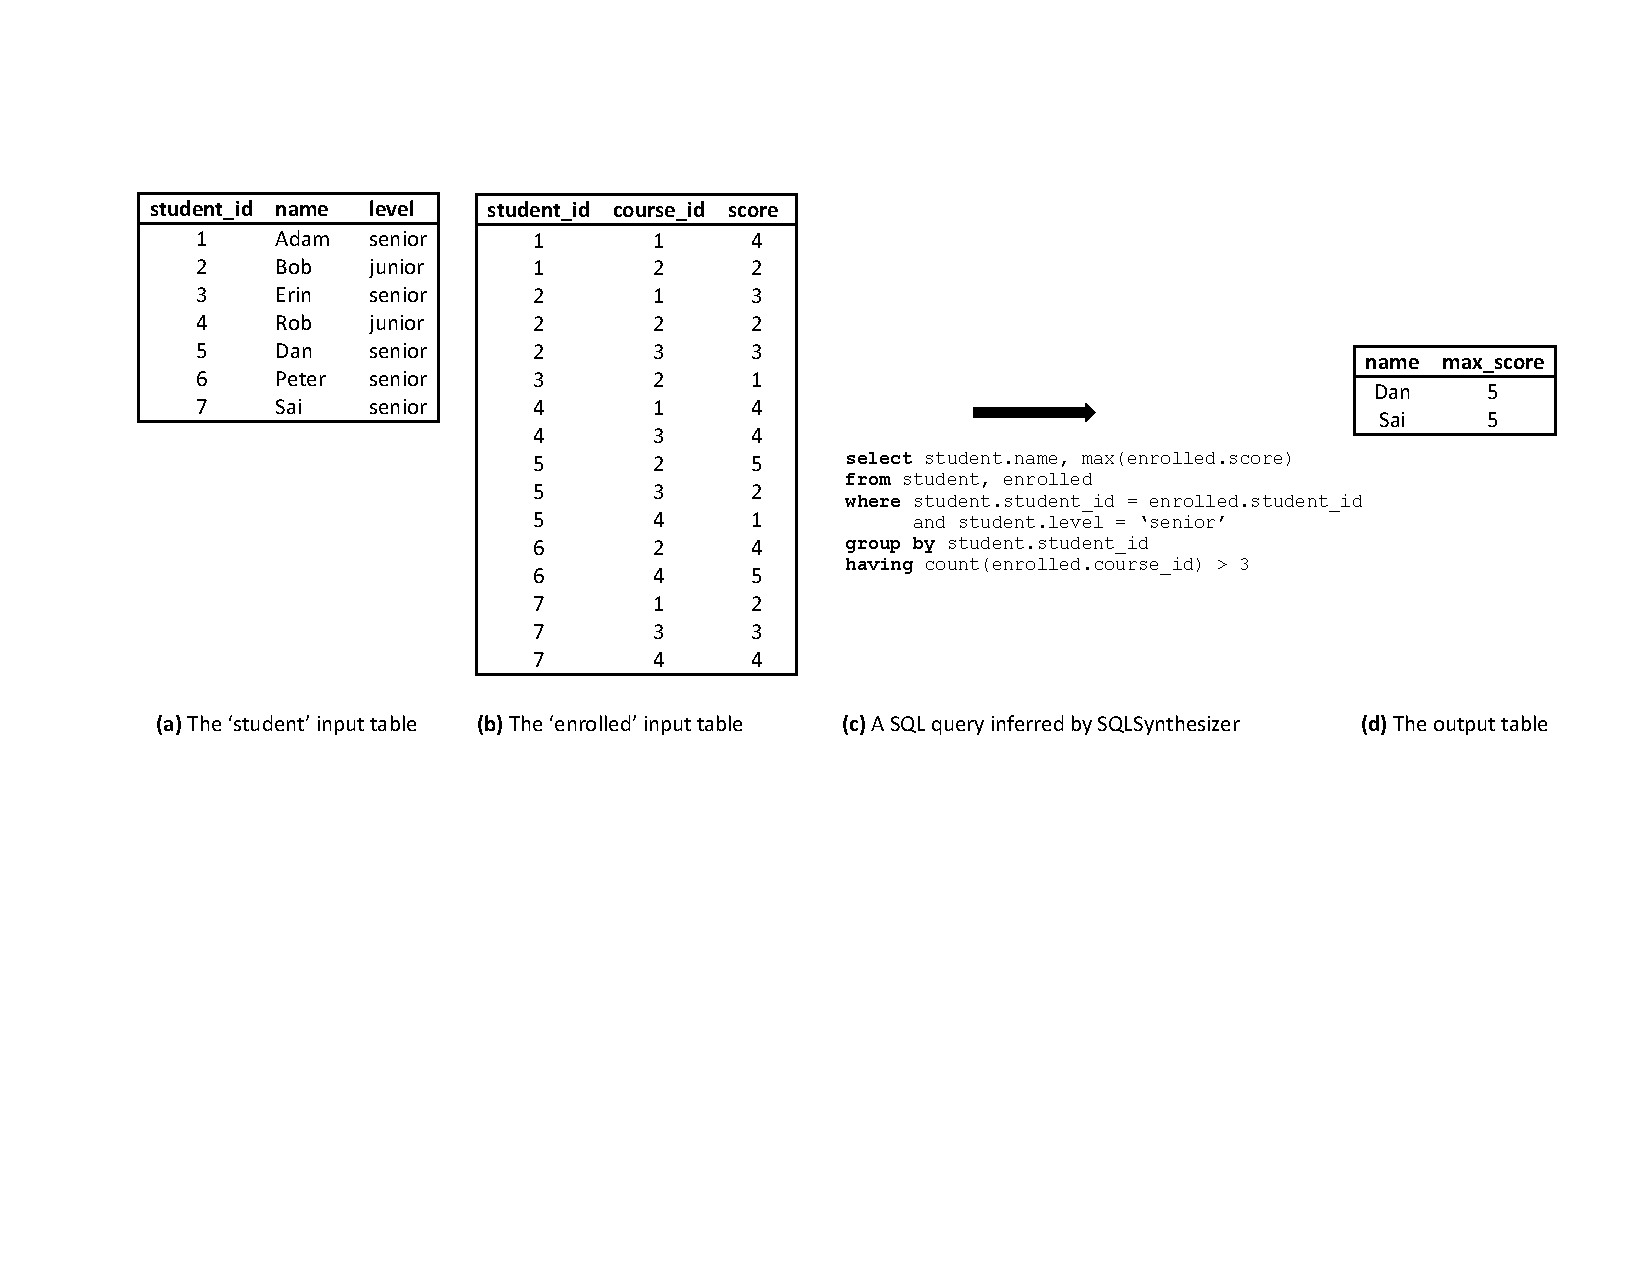
\includegraphics[scale=0.75]{motivating}
  \vspace*{-1.0ex}\caption {{\label{fig:motivating}
  Example input/output tables and the SQL query sythensized by
  \ourtool to solve the problem in Section~\ref{sec:example}. In this example, users provide \ourtool with
  two input tables (shown in (a)) and an output table (shown in (c)).
  \ourtool automatically sythesizes a SQL query (shown in (b)) that
  transforms the two input tables into the output table.
}}
\end{figure*}

\section{Illustrating Example}
\label{sec:example}

We use an example, described below, to illustrate the use
of \ourtool. The example is taken from a classic
database textbook~\cite{cowbook} (Chapter 5, Exercise 1)
and has been simplified for illustration purpose\footnote{
This exercise defines 2 tables: \CodeIn{student}
and \CodeIn{enrolled}. The \CodeIn{student} table
contains three columns: \CodeIn{student\_id}, \CodeIn{name},
and \CodeIn{level}. Table \CodeIn{enrolled} contains
three columns: \CodeIn{student\_id}, \CodeIn{course\_id},
and \CodeIn{score}.
}.

\begin{quote}
\textit{Find the name and the maximum course score of each senior student
enrolled in more than 2 courses.}
\end{quote}

Despite the simplicity of the problem description,
writing a correct SQL query  can be non-trivial for a non-professional
end-user.
Although most users can clearly understand the
question, they must choose the right SQL
features and use them correctly.

Users can use our \ourtool technique to obtain
the desirable query.
As illustrated in Figure~\ref{fig:motivating},
to use \ourtool, an end-user only needs to provide it with
some small, representative example input and output tables
(Figures~\ref{fig:motivating}(a) and~\ref{fig:motivating}(c)).
Then, \ourtool works in a fully-automatic, push-button
way in inferring a SQL query that satisfies the given
example input and output.

 %illustrate in Figure~\ref{fig:motivating}, an alternative
%approach to write this query is to provide \ourtool
%with some representative input-output examples; and
%let \ourtool automatically automatically infer the query.

The SQL query, shown in Figure~\ref{fig:motivating}(b),
first joins two tables on the common \CodeIn{student\_id} column,
and then groups the joined result by the same \CodeIn{student\_id}
column. Further, the query selects all senior
students  (using a query condition in the \CodeIn{WHERE}
clause) who has been enrolled in more than 2 courses
(using a condition in the \CodeIn{HAVING} clause).
Finally, the query projects the result on the
\CodeIn{student.name} column and uses the \CodeIn{MAX} aggregate
to compute the maximum course score.

%the \CodeIn{student} with \CodeIn{enrolled} tables,
%then group bys the joined table by the \CodeIn{student\_id}
%column, and selects students enrolled in more
%than 2 courses (using the \CodeIn{having} statement).
%After that, the query further selects students
%whose level is \CodeIn{senior} and uses the \CodeIn{max}
%aggregator function to compute the maximum course score.
%\todo{the above needs polish}






